
\section{Message Integrity}

The goal of message integrity is integrity, that is, the information must be protected against any malicious modification.

\subsection{MACs}

\subsubsection{MAC Framework}

\begin{definition}[MAC] MAC:

    MAC I=(S,V) defined over (K,M,T) is a pair of algorithms:
    \begin{itemize} [itemsep=2pt,topsep=0pt,parsep=0pt]
        \item Signing Function: S(k,m) outputs a tag t in time T
        \item Verification Function: V(k,m,t) outputs 'yes' or 'no'
    \end{itemize}
    
\end{definition}

The basic framework of MAC is shown in Figure \ref{fig: Lecture 4: MAC FrameWork}.

\begin{figure}[h]
    \centering
    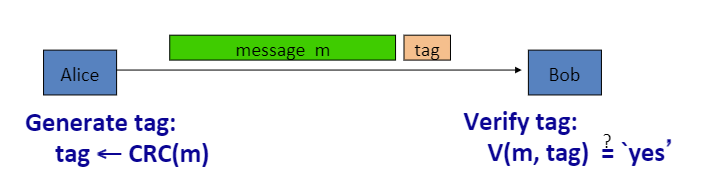
\includegraphics[width=0.8\textwidth]{Stanford_Crypto_1/fig/04_Integrity/MAC Frame Work.png}
    \caption{MAC FrameWork}
    \label{fig: Lecture 4: MAC FrameWork}
\end{figure}


\subsection{Secure MAC}

\subsubsection{Attackers in MACs}

Attacker's Power: chosen message attack, that is attacker can given $m_1, m_2, \cdots, m_q$, and an oracle will give back $\mathrm{t}_{\mathrm{i}} \leftarrow \mathrm{s}\left(\mathrm{k}, \mathrm{m}_{\mathrm{i}}\right)$.

Attacker's Goal: existential forgery, that is to produce some new valid message/tag pair (m,t), $(\mathrm{m}, \mathrm{t}) \notin\left\{\left(\mathrm{m}_{1}, \mathrm{t}_{1}\right), \ldots,\left(\mathrm{m}_{\mathrm{q}}, \mathrm{t}_{\mathrm{q}}\right)\right\}$.


\subsubsection{Motivation of Secure MAC}

intuitively, we have two expectations, A secure MAC should be able to:
\begin{enumerate} [itemsep=2pt,topsep=0pt,parsep=0pt]
    \item an attacker cannot produce a valid tag for a new message,  even for a gibberish message
    \item given (m,t), attacker cannot even produce (m,t') for $t' \neq t$
\end{enumerate}

\subsubsection{Definition of Secure MAC}

A game in MAC is defined as in Figure \ref{fig: Lecture 4: Game for MAC}.

\begin{figure}[h]
    \centering
    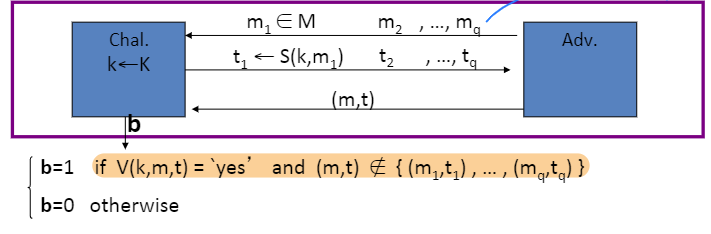
\includegraphics[width=0.8\textwidth]{Stanford_Crypto_1/fig/04_Integrity/Game for MAC.png}
    \caption{Game for MAC}
    \label{fig: Lecture 4: Game for MAC}
\end{figure}

One thing should be notice that, here, the adversary actually do not know the Ciphertext.

So we can generate the following definition of \textbf{secure MAC}
 
\begin{definition} [Secure MAC] Secure MAC

    I=(S,V) is a \textbf{secure MAC} if for  all "efficient" A, 
    $$
    \operatorname{Adv}_{\mathrm{MAC}}[A, I]=\operatorname{Pr}[\text { Chal. outputs } 1] \quad \text { is "negligible." }
    $$
\end{definition}


\section{Collision Resistance}

\subsection{Introduction}

Here are the definitions of \textbf{collision} and \textbf{collision resistant}.

\begin{definition} [collision and collision resistant] collision and collision resistant:

    Let $H: M \rightarrow T$ be a hash function $\quad(|M|>>|T|)$
    A collision for $\mathrm{H}$ is a pair $\mathrm{m}_{0}, \mathrm{~m}_{1} \in \mathrm{M}$ such that:
    $$
    \mathrm{H}\left(\mathrm{m}_{0}\right)=\mathrm{H}\left(\mathrm{m}_{1}\right) \text { and } \mathrm{m}_{0} \neq \mathrm{m}_{1}
    $$
    A function $\mathrm{H}$ is collision resistant if for all (explicit) "eff" algs. A:
    $\operatorname{Adv}_{\mathrm{CR}}[\mathrm{A}, \mathrm{H}]=\operatorname{Pr}[\mathrm{A}$ outputs collision for $\mathrm{H}]$
    is "neg".
    
\end{definition}

\subsection{Generic Birthday Attack}

\subsubsection{Generic Attack on C.R. functions}

\begin{method} [Generic Attack] Generic Attack:

\begin{enumerate} [itemsep=2pt,topsep=0pt,parsep=0pt]
    \item Choose $2^{n / 2}$ random messages in $M$ : $m_{1}, \ldots, m_{2}^{n / 2} \quad$ (distinct w.h.p)
    \item For $\mathrm{i}=1, \ldots, 2^{\mathrm{n} / 2}$ compute $\mathrm{t}_{\mathrm{i}}=\mathrm{H}\left(\mathrm{m}_{\mathrm{i}}\right) \quad \in\{0,1\}^{\mathrm{n}}$
    \item Look for a collision $\left(t_{i}=t_{j}\right)$. If not found, got back to step 1 .
\end{enumerate}

\end{method}

The time complexity of this method is $\mathcal{O}(2^{n/2})$

\subsubsection{The Birthday Paradox}

\begin{theorem} [The Birthday Paradox] The Birthday Paradox:

    when $\mathrm{n}=1.2 \times \mathrm{B}^{1 / 2}$ then $\operatorname{Pr}\left[\exists \mathrm{i} \neq \mathrm{j}: \mathrm{r}_{\mathrm{i}}=\mathrm{r}_{\mathrm{j}}\right] \geq 1 / 2$
\end{theorem}

\textbf{Notes:} If the distribution is uniform distribution, than it is the best case. Other distribution will lead to worse case.

The birthday paradox is illustrated in Figure \ref{fig: Lecture 4: The Birthday Paradox}.

\begin{figure}[h]
    \centering
    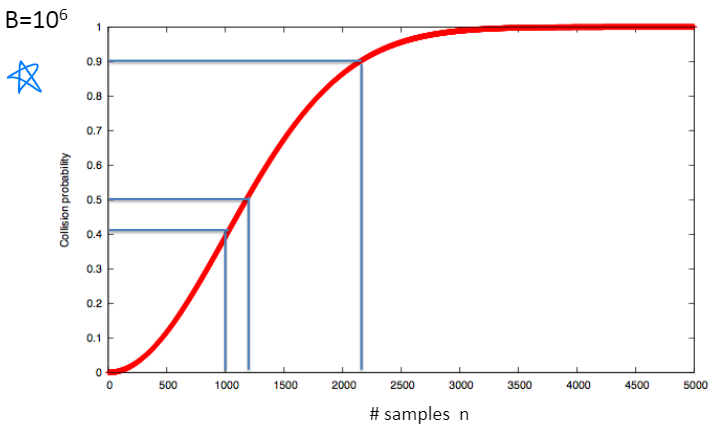
\includegraphics[width=0.8\textwidth]{Stanford_Crypto_1/fig/04_Integrity/The birthday paradox.png}
    \caption{The Birthday Paradox}
    \label{fig: Lecture 4: The Birthday Paradox}
\end{figure}

Based on the birthday paradox, if we use the generic attack, the expected number of iteration is roughly equal to 2.

\section{Construction of Collision Resistance}

The construction will be divided into two steps:

\begin{enumerate} [itemsep=2pt,topsep=0pt,parsep=0pt]
    \item given C.R. function for short messages, we can construct C.R. function for long messages. (The Merkle-Damagard Paradigm). That is, if we can find a C.R. compression function, then we can build a C.R. Hash function.
    \item Then we will propose some method to build C.R. compression function
\end{enumerate}

\subsection{The Merkle-Damagard Paradigm}

The structure of the Merkle-Damagard Paradigm is shown in Figure \ref{fig: Lecture 4: MD Framework}.

\begin{figure}[h]
    \centering
    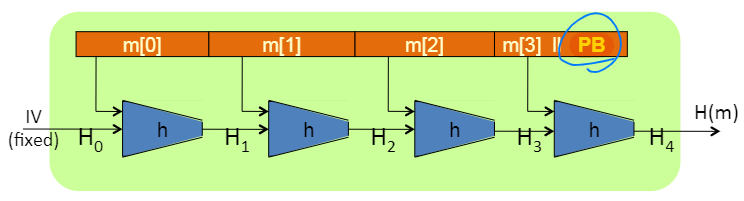
\includegraphics[width=0.8\textwidth]{Stanford_Crypto_1/fig/04_Integrity/MD iterated construction.png}
    \caption{MD Framework}
    \label{fig: Lecture 4: MD Framework}
\end{figure}

That is given $\mathrm{h}: \mathrm{T} \times \mathrm{X} \rightarrow \mathrm{T} \quad$ (compression function), we obtain $\mathrm{H}: \mathrm{X}^{\leq \mathrm{L}} \longrightarrow \mathrm{T} . \quad$ ($\mathrm{H}_{\mathrm{i}}-$chaining variables).

The \textbf{PB} part is the padding block. [10000$\cdots$000 || msg\_len(64-bits)]. If no space for PB, then add another block.

Based on Merkle-Damagard Paradigm, we have a theorem

\begin{theorem} [MD Collision Resistance] MD Collision Resistance:

    If h is C.R., then so is H
    
\end{theorem}

The proof is quite simple from final part and rollback.

\textbf{Notes: } The MD C.R. theorem told us, if we want to construct C.R. function, suffices to construct compression function.


\subsection{Constructing Compression Functions}

\subsubsection{Construct Compression Function from Block Cipher}

One method called \textbf{Davies-Meyer} Method: $\mathrm{h}(\mathrm{H}, \mathrm{m})=\mathrm{E}(\mathrm{m}, \mathrm{H}) \oplus \mathrm{H}$  and is shown in Figure \ref{fig: Lecture 4: Davies_Meyer Method}.

\begin{figure}[h]
    \centering
    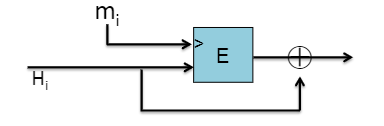
\includegraphics[width=0.5\textwidth]{Stanford_Crypto_1/fig/04_Integrity/Davies_Meyer Method.png}
    \caption{Davies\_Meyer Method}
    \label{fig: Lecture 4: Davies_Meyer Method}
\end{figure}

\begin{theorem}
    Suppose $E$ is an ideal cipher (collection of $|K|$ random perms.). Finding a collision $\mathrm{h}(\mathrm{H}, \mathrm{m})=\mathrm{h}\left(\mathrm{H}^{\prime}, \mathrm{m}^{\prime}\right)$ takes $\mathrm{O}\left(2^{n / 2}\right)$ evaluations of $(\mathrm{E}, \mathrm{D})$.
\end{theorem}

One application of the Davies-Meyer method is the SHA-256, which is shown in Figure \ref{fig: Lecture 4: SHA256 DM Method}.

\begin{figure}[h]
    \centering
    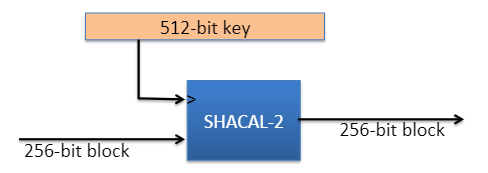
\includegraphics[width=0.5\textwidth]{Stanford_Crypto_1/fig/04_Integrity/SHA256 DM Method.png}
    \caption{SHA256 DM Method}
    \label{fig: Lecture 4: SHA256 DM Method}
\end{figure}


\subsubsection{Provable Compression functions}

\begin{method} [Provable Compression functions] Provable Compression functions: 

    Choose a random 2000-bit prime $p$ and random $1 \leq u, v \leq p$.
    For $m, h \in\{0, \ldots, p-1\} \quad$ define $\quad h(H, m)=u^{H} \cdot v^{m} \quad(\bmod p)$
\end{method}

\textbf{Fact: } finding collision for h is as hard as solving "discrete-log" module p. The problem of this method is that it is too slow.



\section{MACs based on PRFs}

\subsubsection{Property}

\begin{theorem} [From Secure PRF to Secure MAC] From Secure PRF to Secure MAC:

    If $\mathrm{F}: \mathrm{K} \times \mathrm{X} \rightarrow \mathrm{Y}$ is a secure PRF and $1 /|\mathrm{Y}|$ is negligible (i.e. $|Y|$ is large) then $I_{F}$ is a secure MAC.
    
    In particular, for every eff. MAC adversary A attacking $I_F$ there exists an eff. PRF adversary B attacking F s.t.:
    $$
    \operatorname{Adv}_{\mathrm{MAC}}\left[\mathrm{A}, \mathrm{I}_{F}\right] \leq \operatorname{Adv}_{\mathrm{PRF}}[\mathrm{B}, \mathrm{F}]+1 /|\mathrm{Y}|
    $$
    
\end{theorem}

\textbf{Notes: $I_F$ is secure as long as $|Y|$ is large}

And we can regard \textbf{AES} as a MAC for 16-byte messages.

\subsubsection{Motivation}

Given a PRF for short messages (AES), construct a PRF for long messages.


\subsection{ECBC-MAC}

The structure of ECBC-MAC is shown in Figure \ref{fig: Lecture 4: ECBC-MAC Structure}.

\begin{figure}[h]
    \centering
    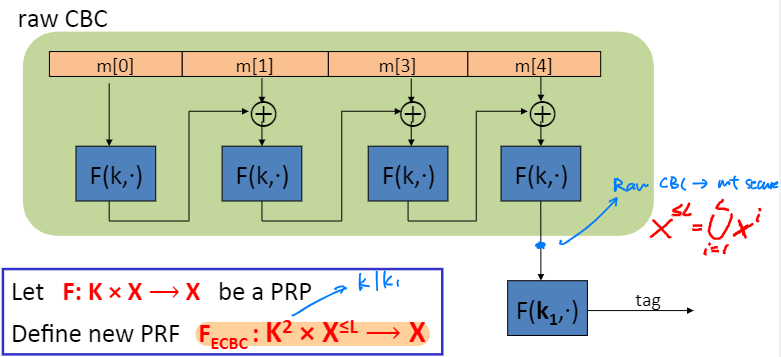
\includegraphics[width=0.8\textwidth]{Stanford_Crypto_1/fig/04_Integrity/CBC_MAC Structure.png}
    \caption{ECBC-MAC Structure}
    \label{fig: Lecture 4: ECBC-MAC Structure}
\end{figure}


One problem is Why the last Encryption step in ECBC-MAC?

Suppose we define a MAC $I_{\text {RAW }}=(S, V) \quad$ where
$$
S(k, m)=\operatorname{rawCBC}(k, m)
$$
Then $I_{\text {RAW }}$ is easily broken using a 1-chosen msg attack.

Adversary works as follows:
\begin{enumerate} [itemsep=2pt,topsep=0pt,parsep=0pt]
    \item choose an arbitrary one-block message $m \in X$
    \item request tag for m, Get $t=F(k,m)$
    \item Output t as MAC forgery for the 2-block message (m, t $\oplus$ m)
\end{enumerate}


Then the adversary win the challenge: $\operatorname{rawCBC}(k,(m, t \oplus m))=F(k, F(k, m) \oplus(t \oplus m))=F(k, t \oplus(t \oplus m))=t$

\subsubsection{CBC-MAC Padding}

For security, padding must be invertible, i.e.  $m_{0} \neq m_{1} \Rightarrow \quad \operatorname{pad}\left(m_{0}\right) \neq \operatorname{pad}\left(m_{1}\right)$.

The first method is the \textbf{ISO} standard: pad with "1000...00". Add new dummy block if needed. The " 1 " indicates beginning of pad. The structure of the ISO standard padding is shown in Figure \ref{fig: Lecture 4: ISO CBC Padding}.


\begin{figure}[h]
    \centering
    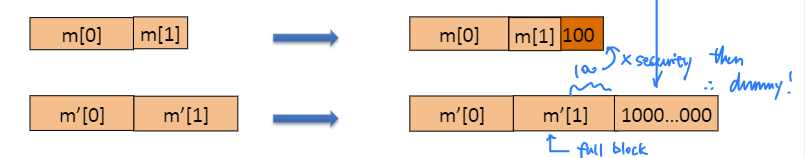
\includegraphics[width=0.8\textwidth]{Stanford_Crypto_1/fig/04_Integrity/ISO CBC Padding.png}
    \caption{ISO CBC Padding}
    \label{fig: Lecture 4: ISO CBC Padding}
\end{figure}


The second method is the \textbf{NIST} standard: it use a key tuple: $key=(k,k_1,k_2)$, in which, $(k_1,k_2)$ are derived from k. From this standard, we do not need the final encryption step of ECBC, and we do not need dummy block. The structure of the NIST standard padding is shown in Figure \ref{fig: Lecture 4: NIST CBC Padding}.

\begin{figure}[h]
    \centering
    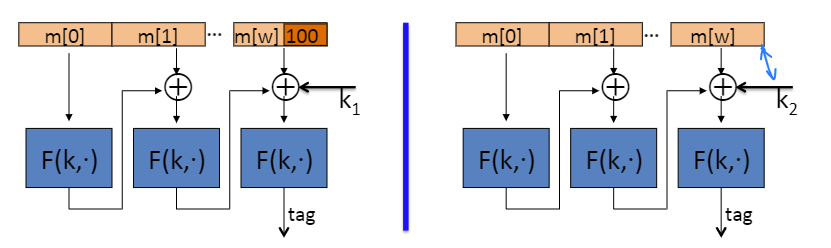
\includegraphics[width=0.8\textwidth]{Stanford_Crypto_1/fig/04_Integrity/NIST CBC Padding.png}
    \caption{NIST CBC Padding}
    \label{fig: Lecture 4: NIST CBC Padding}
\end{figure}

\subsubsection{Randomize MAC}

Another form of MAC with better security is shown in Figure \ref{fig: Lecture 4: Randomize MAC}

\begin{figure}[h]
    \centering
    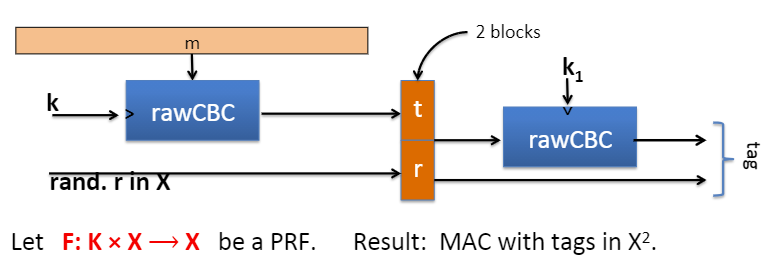
\includegraphics[width=0.8\textwidth]{Stanford_Crypto_1/fig/04_Integrity/Randomize MAC.png}
    \caption{Randomize MAC}
    \label{fig: Lecture 4: Randomize MAC}
\end{figure}

The security of this method is:  $A d v_{\mathrm{MAC}}\left[A, I_{\mathrm{RCBC}}\right] \leq A d v_{\mathrm{PRP}}[B, F] \cdot\left(1+2 q^{2} /|X|\right)$


\subsection{NMAC}

The structure of NMAC is shown in Figure \ref{fig: Lecture 4: NMAC Structure}.

\begin{figure}[h]
    \centering
    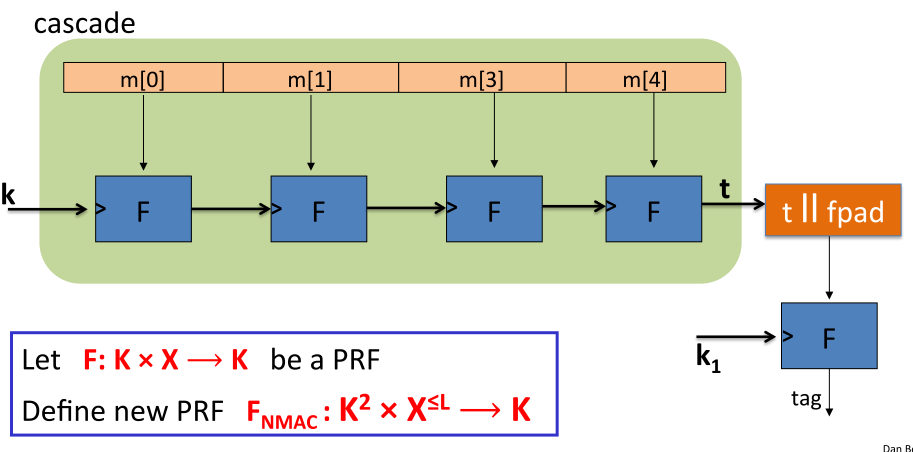
\includegraphics[width=0.8\textwidth]{Stanford_Crypto_1/fig/04_Integrity/NMAC Structure.png}
    \caption{NMAC Structure}
    \label{fig: Lecture 4: NMAC Structure}
\end{figure}

\subsection{Security Analysis of ECBC-MAC and NMAC}


\begin{theorem} [Security of ECBC-MAC and NMAC] Security of ECBC-MAC and NMAC:

    For any $L>0$,
    For every eff. q-query PRF adv. A attacking $F_{E C B C}$ or $F_{\text {NMAC }}$ there exists an eff. adversary B s.t.:
    $$
    \begin{aligned}
    &\operatorname{Adv}_{\mathrm{PRF}}\left[A, F_{\mathrm{ECBC}}\right] \leq \operatorname{Adv}_{\mathrm{PRP}}[B, F]+2 q^{2} /|X| \\
    &\operatorname{Adv}_{\mathrm{PRF}}\left[A, F_{\mathrm{NMAC}}\right] \leq q \cdot L \cdot \operatorname{Adv}_{\mathrm{PRF}}[B, F]+q^{2} / 2|K|
    \end{aligned}
    $$

\end{theorem}

\textbf{Notes:} CBC-MAC is secure as long as $q \ll<|X|^{1 / 2}$ NMAC is secure as long as $q<|K|^{1 / 2}$

An example using this theorem:

Suppose we want $\operatorname{Adv}_{\mathrm{PRF}}\left[\mathrm{A}, \mathrm{F}_{\mathrm{ECBC}}\right] \leq 1 / 2^{32} \Leftrightarrow \mathrm{q}^{2} /|\mathrm{X}|<1 / 2^{32}$
Then for AES: $|X|=2^{128} \Rightarrow q<2^{48}$
So, after $2^{48}$ messages must, must change key\

\subsubsection{Comparison of ECBC-MAC and NMAC}

ECBC-MAC is commonly used as an AES-based MAC.

NMAC not usually used with AES or 3DES. Main reason is: it need to change AES key on every block, requires re-computing AES key expansion.


\subsection{PMAC}

The structure of paralle MAC (PMAC) is shown in Figure \ref{fig: Lecture 4: PMAC Structure}

\begin{figure}[h]
    \centering
    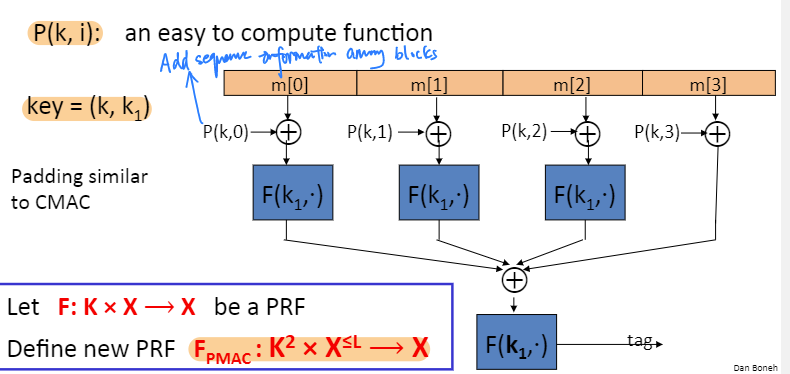
\includegraphics[width=0.8\textwidth]{Stanford_Crypto_1/fig/04_Integrity/PMAC_Structure.png}
    \caption{PMAC Structure}
    \label{fig: Lecture 4: PMAC Structure}
\end{figure}


\subsubsection{Property of PMAC}

PMAC is \textbf{incremental}. Which means we can easily generate a new tag when only one part of the PMAC is changed. For example when $m[1] \leftarrow m'[1]$, we can just do $\mathrm{F}^{-1}\left(\mathrm{k}_{1}, \mathrm{tag}\right) \oplus \mathrm{F}\left(\mathrm{k}_{1}, \mathrm{~m}[1] \oplus \mathrm{P}(\mathrm{k}, 1)\right) \oplus \mathrm{F}\left(\mathrm{k}_{1}, \mathrm{~m}^{\prime}[1] \oplus \mathrm{P}(\mathrm{k}, 1)\right)$


\subsubsection{Security Analysis}

\begin{theorem} [Security of PMAC] Security of PMAC:

    For any $L>0$,
    If $F$ is a secure PRF over $(K, X, X)$ then
    $F_{P M A C}$ is a secure PRF over $(K, X \leq L, X)$.
    For every eff. q-query PRF adv. A attacking $F_{\text {PMAC }}$ there exists an eff. PRF adversary B s.t.:
    $\operatorname{Adv}_{\mathrm{PRF}}\left[\mathrm{A}, \mathrm{F}_{\mathrm{PMAC}}\right] \leq \operatorname{Adv}_{\mathrm{PRF}}[\mathrm{B}, \mathrm{F}]+2 \mathrm{q}^{2} \mathrm{~L}^{2} /|\mathrm{X}|$
    
\end{theorem}


From the theorem, we knows that: PMAC is secure as long as $q L \ll|X|^{1 / 2}$.


\subsection{Carter-Wegman MAC}

\subsubsection{One-time MAC}



\section{MACs from Collision Resistance}

\subsection{HMAC}

The HMAC method need two dependent keys and an IV. The structure of HMAC is shown in Figure \ref{fig: Lecture 4: HMAC Structure}. It can be presented by:


$$
\quad S(k, m)=H(k \oplus o p a d \| H(k \oplus i p a d \| m))
$$

\begin{figure}[h]
    \centering
    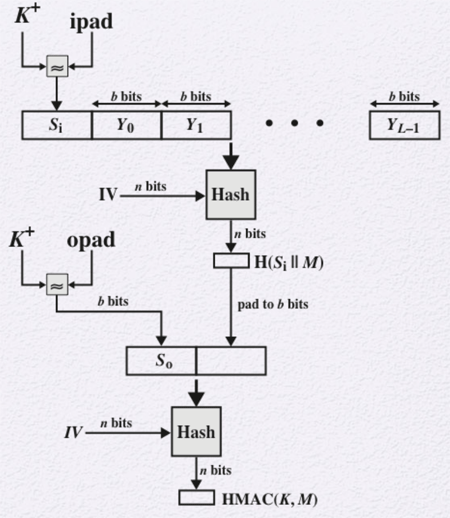
\includegraphics[width=0.5\textwidth]{Stanford_Crypto_1/fig/04_Integrity/HMAC Structure.png}
    \caption{HMAC Structure}
    \label{fig: Lecture 4: HMAC Structure}
\end{figure}

\subsubsection{Properties:}

HMAC is assumed to be a secure PRF
\begin{itemize} [itemsep=2pt,topsep=0pt,parsep=0pt]
    \item Can be proven under certain PRF assumptions about h(.,.)
    \item Security bounds similar to NMAC: Need $q^{2} /|T|$ to be negligible $\left(q<|T|^{1 / 2}\right)$
\end{itemize}

\section{Timing Attacks on MAC Verification}

Timing attacks try to use the step of Verification of the HMAC, because originally the earlier byte will be test first. So based on the feedback timing, some attacker try to find the real MAC.

So the lesson is \textbf{Don't implement crypto yourself}.


\section{Summary}
In this chapter, we first introduce what is an MAC, and we defined what is a secure MAC. The basic intuition is "the adversary cannot build a new (m,t) pair that is available".

Then we defined what is collision resistant and how to build collision resistant function from compression function and how to build compression function from Block Cipher. We also declared that we can regard AES as a PRF.

Then we illustrate three method for building MAC based on PRFs:  ECBC-MAC and NMAC and PMAC. And based on previous discussion of collision resistant function, we discussed the MAC based on collision resistant Hash Function: HMAC.
